% Options for packages loaded elsewhere
\PassOptionsToPackage{unicode}{hyperref}
\PassOptionsToPackage{hyphens}{url}
\PassOptionsToPackage{dvipsnames,svgnames,x11names}{xcolor}
\PassOptionsToPackage{space}{xeCJK}
\documentclass[
  10pt,
]{article}
\usepackage{xcolor}
\usepackage[margin=0.7in]{geometry}
\usepackage{amsmath,amssymb}
\setcounter{secnumdepth}{-\maxdimen} % remove section numbering
\usepackage{iftex}
\ifPDFTeX
  \usepackage[T1]{fontenc}
  \usepackage[utf8]{inputenc}
  \usepackage{textcomp} % provide euro and other symbols
\else % if luatex or xetex
  \usepackage{unicode-math} % this also loads fontspec
  \defaultfontfeatures{Scale=MatchLowercase}
  \defaultfontfeatures[\rmfamily]{Ligatures=TeX,Scale=1}
\fi
\usepackage{lmodern}
\ifPDFTeX\else
  % xetex/luatex font selection
  \setmainfont[]{Arial}
  \setmonofont[]{Consolas}
  \ifXeTeX
    \usepackage{xeCJK}
    \setCJKmainfont[]{Microsoft YaHei}
  \fi
  \ifLuaTeX
    \usepackage[]{luatexja-fontspec}
    \setmainjfont[]{Microsoft YaHei}
  \fi
\fi
% Use upquote if available, for straight quotes in verbatim environments
\IfFileExists{upquote.sty}{\usepackage{upquote}}{}
\IfFileExists{microtype.sty}{% use microtype if available
  \usepackage[]{microtype}
  \UseMicrotypeSet[protrusion]{basicmath} % disable protrusion for tt fonts
}{}
\makeatletter
\@ifundefined{KOMAClassName}{% if non-KOMA class
  \IfFileExists{parskip.sty}{%
    \usepackage{parskip}
  }{% else
    \setlength{\parindent}{0pt}
    \setlength{\parskip}{6pt plus 2pt minus 1pt}}
}{% if KOMA class
  \KOMAoptions{parskip=half}}
\makeatother
\usepackage{longtable,booktabs,array}
\usepackage{calc} % for calculating minipage widths
% Correct order of tables after \paragraph or \subparagraph
\usepackage{etoolbox}
\makeatletter
\patchcmd\longtable{\par}{\if@noskipsec\mbox{}\fi\par}{}{}
\makeatother
% Allow footnotes in longtable head/foot
\IfFileExists{footnotehyper.sty}{\usepackage{footnotehyper}}{\usepackage{footnote}}
\makesavenoteenv{longtable}
\usepackage{graphicx}
\makeatletter
\newsavebox\pandoc@box
\newcommand*\pandocbounded[1]{% scales image to fit in text height/width
  \sbox\pandoc@box{#1}%
  \Gscale@div\@tempa{\textheight}{\dimexpr\ht\pandoc@box+\dp\pandoc@box\relax}%
  \Gscale@div\@tempb{\linewidth}{\wd\pandoc@box}%
  \ifdim\@tempb\p@<\@tempa\p@\let\@tempa\@tempb\fi% select the smaller of both
  \ifdim\@tempa\p@<\p@\scalebox{\@tempa}{\usebox\pandoc@box}%
  \else\usebox{\pandoc@box}%
  \fi%
}
% Set default figure placement to htbp
\def\fps@figure{htbp}
\makeatother
\setlength{\emergencystretch}{3em} % prevent overfull lines
\providecommand{\tightlist}{%
  \setlength{\itemsep}{0pt}\setlength{\parskip}{0pt}}
\usepackage{bookmark}
\IfFileExists{xurl.sty}{\usepackage{xurl}}{} % add URL line breaks if available
\urlstyle{same}
\hypersetup{
  colorlinks=true,
  linkcolor={Maroon},
  filecolor={Maroon},
  citecolor={Blue},
  urlcolor={blue},
  pdfcreator={LaTeX via pandoc}}

\author{}
\date{}

\usepackage{float}
\usepackage{needspace}
\setCJKmonofont{Microsoft YaHei}
\Urlmuskip=0mu plus 2mu\relax
\begin{document}

\section{Training continuation and quality-related
errors}\label{training-continuation-and-quality-related-errors}

November 15, 2026 · \href{quality-and-training.zh.md}{中文} ·
\href{quality-and-training.en.pdf}{English PDF}

Errors on the expanded dataset do not follow a simple pattern of
increasing concentration at lower quality. Too few real poor-quality
cases contribute to the uncertainty, but stronger direct evidence
concerns their disease-label imbalance, differences between source
quality standards, and substantial error-ranking information already
present in disease scores. Current development results do not establish
a stable additional review benefit from quality scores.

Six training conditions with three common seeds are now running, with
2,400 successful optimizer updates planned per run. This report records
their status and the analysis of quality-related errors, following the
\href{../2026-11-13/README.en.md}{November 13 experiments}.

Both earlier disease models, the original quality model, and the EyeQ
quality model completed 20 epochs, as recorded in the
\href{../2026-11-12/training-progress.en.md}{November 12 report}. All
four November 13 fixed-budget experiments are also complete. Review
boundaries and final testing await model and rule selection.

\subsection{Data and the proposal}\label{data-and-the-proposal}

The \href{../../../proposal-1106.pdf}{original proposal} asks whether
glaucoma score p and quality score q can jointly define a review region.
It does not guarantee that errors will cluster at low q. The relevant
test is whether adding q selects more errors and misses than p alone at
the same review volume.

The primary analysis uses 2,053 rule-development originals from frozen
release expanded\_20261113: 814 positives, 1,239 negatives, and 1,917
linked groups. Linked groups keep confirmed paired eyes, repeat
photographs, and related image versions together for split assignment
and statistical resampling. Disease scores come from the update-1,200
budget-end checkpoint of the 50\% mixed-degradation arm. Quality scores
come from the selected FTHNet-distilled student checkpoint. This student
is trained to reproduce an existing quality model's continuous scores,
with larger values indicating better predicted quality. A separate
2,046-image model-validation set checks the distribution; the EyeQ
quality model is also evaluated on these same 4,099 originals. Model
validation has already informed checkpoint selection, and rule
development supports this exploratory analysis. Held-out final tests
have not been scored.

The display decision calls an image positive when p exceeds 0.5. This
yields 124/814 missed positives and 84/1,239 false alarms on rule
development. Sources retain their own disease definitions, including
AIROGS referral labels and other sources' diagnosis labels;
within-source results explain differences.

\subsection{Counts, rates, and disease
classes}\label{counts-rates-and-disease-classes}

\Needspace{9\baselineskip}
\begin{longtable}[]{@{}
  >{\raggedright\arraybackslash}p{(\linewidth - 8\tabcolsep) * \real{0.2000}}
  >{\raggedright\arraybackslash}p{(\linewidth - 8\tabcolsep) * \real{0.2000}}
  >{\raggedright\arraybackslash}p{(\linewidth - 8\tabcolsep) * \real{0.2000}}
  >{\raggedright\arraybackslash}p{(\linewidth - 8\tabcolsep) * \real{0.2000}}
  >{\raggedright\arraybackslash}p{(\linewidth - 8\tabcolsep) * \real{0.2000}}@{}}
\toprule\noalign{}
\begin{minipage}[b]{\linewidth}\raggedright
q interval
\end{minipage} & \begin{minipage}[b]{\linewidth}\raggedright
Images
\end{minipage} & \begin{minipage}[b]{\linewidth}\raggedright
Misses / positives
\end{minipage} & \begin{minipage}[b]{\linewidth}\raggedright
False alarms / negatives
\end{minipage} & \begin{minipage}[b]{\linewidth}\raggedright
Error rate
\end{minipage} \\
\midrule\noalign{}
\endhead
\bottomrule\noalign{}
\endlastfoot
0--0.2 & 49 & 3/26 & 1/23 & 8.2\% \\
0.2--0.4 & 305 & 13/134 & 19/171 & 10.5\% \\
0.4--0.6 & 757 & 50/349 & 29/408 & 10.4\% \\
0.6--0.8 & 777 & 48/268 & 31/509 & 10.2\% \\
0.8--1 & 165 & 10/37 & 4/128 & 8.5\% \\
\end{longtable}

\begin{figure}[H]
\centering
\pandocbounded{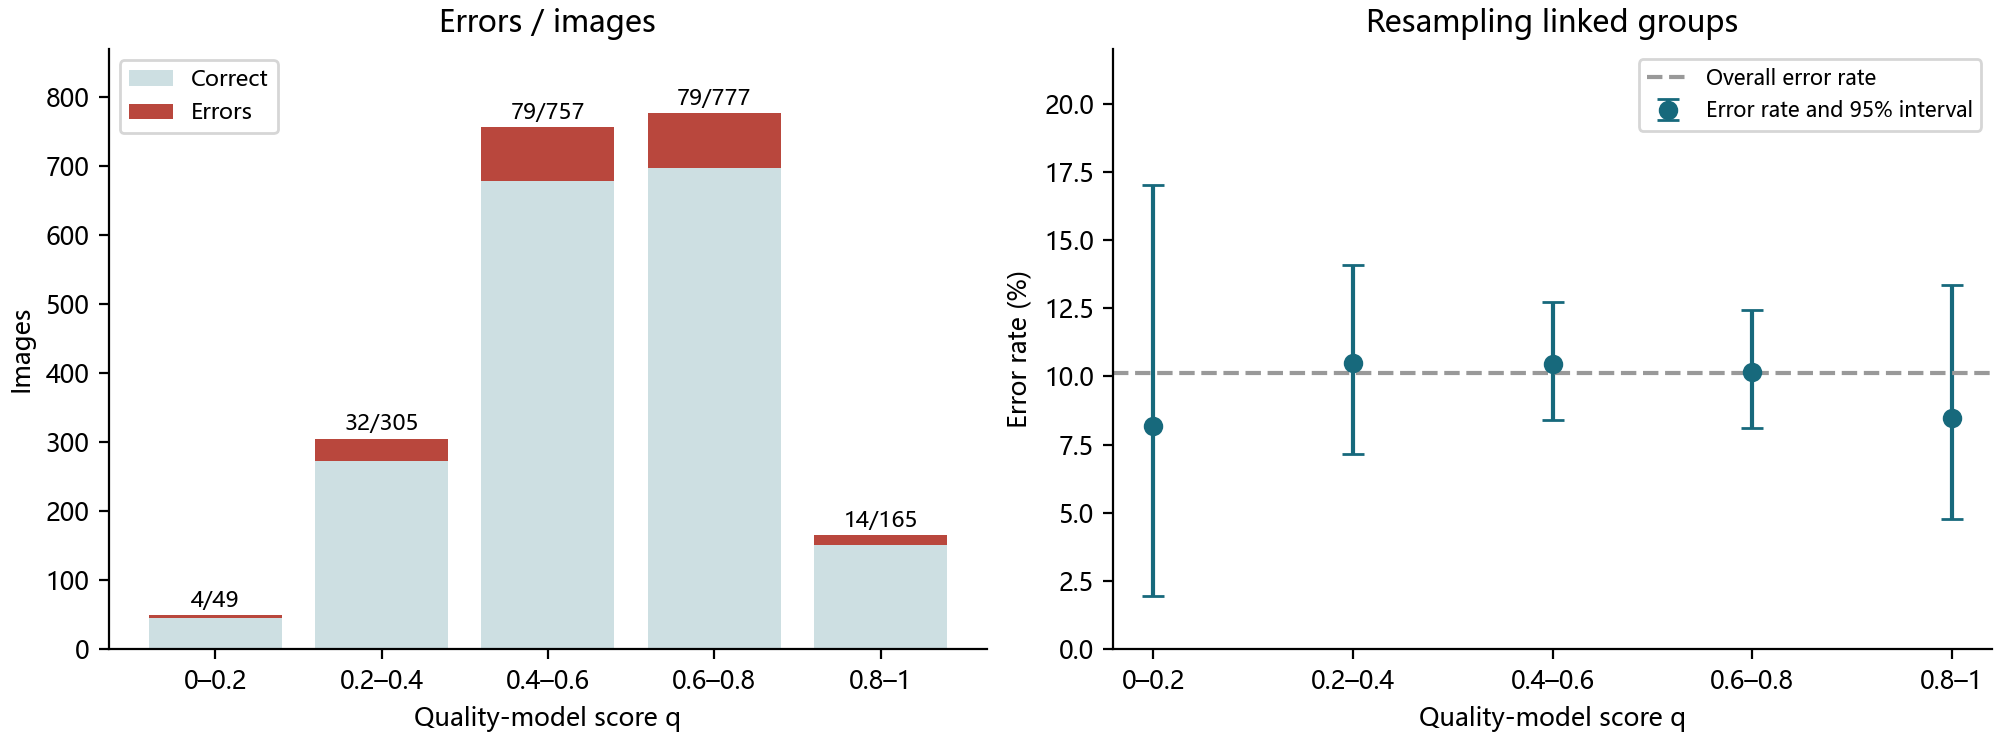
\includegraphics[keepaspectratio,alt={Image counts and error rates within quality-score intervals}]{quality-counts-rates.en.png}}
\caption{Image counts and error rates within quality-score intervals}
\end{figure}

Figure 1 labels errors / images on the left and shows error rates with
95\% intervals from 2,000 linked-group bootstrap samples on the right.
Only 49 images, 2.4\% of rule development, have q below 0.2; four are
errors. Images at q of at least 0.4 account for 82.8\% of photographs
and 82.7\% of errors. More errors in the middle and upper quality ranges
largely follow their greater image counts. Interval-specific error rates
are about 8\%--10\%, without a sustained decline as q rises.

Low q also ranks false alarms and misses in different directions: their
error-ranking AUROCs are 0.5950 and 0.4082, respectively. High q does
not exclude a miss; the q interval 0.8--1 contains 37 positives, with
ten missed. Fifty development errors have p at either extreme, defined
as p at most 0.1 or at least 0.9; 41 have q of at least 0.4. Quality
alone cannot cover these cases.

Error-ranking AUROC means the probability of assigning higher risk to a
randomly selected error than to a randomly selected correct prediction;
0.5 means random ranking. It differs from disease-classification AUROC.
Ranking by low q gives development AUROC 0.5092 {[}0.4703, 0.5476{]} and
model-validation AUROC 0.5238. The original-data control gives 0.5683,
expanded clean 0.5111, 30\% degradation 0.5154, and 50\% degradation
0.5092. The change already appears without augmentation, so degradation
alone does not explain it.

\subsection{Human quality grades and score
scales}\label{human-quality-grades-and-score-scales}

\begin{figure}[H]
\centering
\pandocbounded{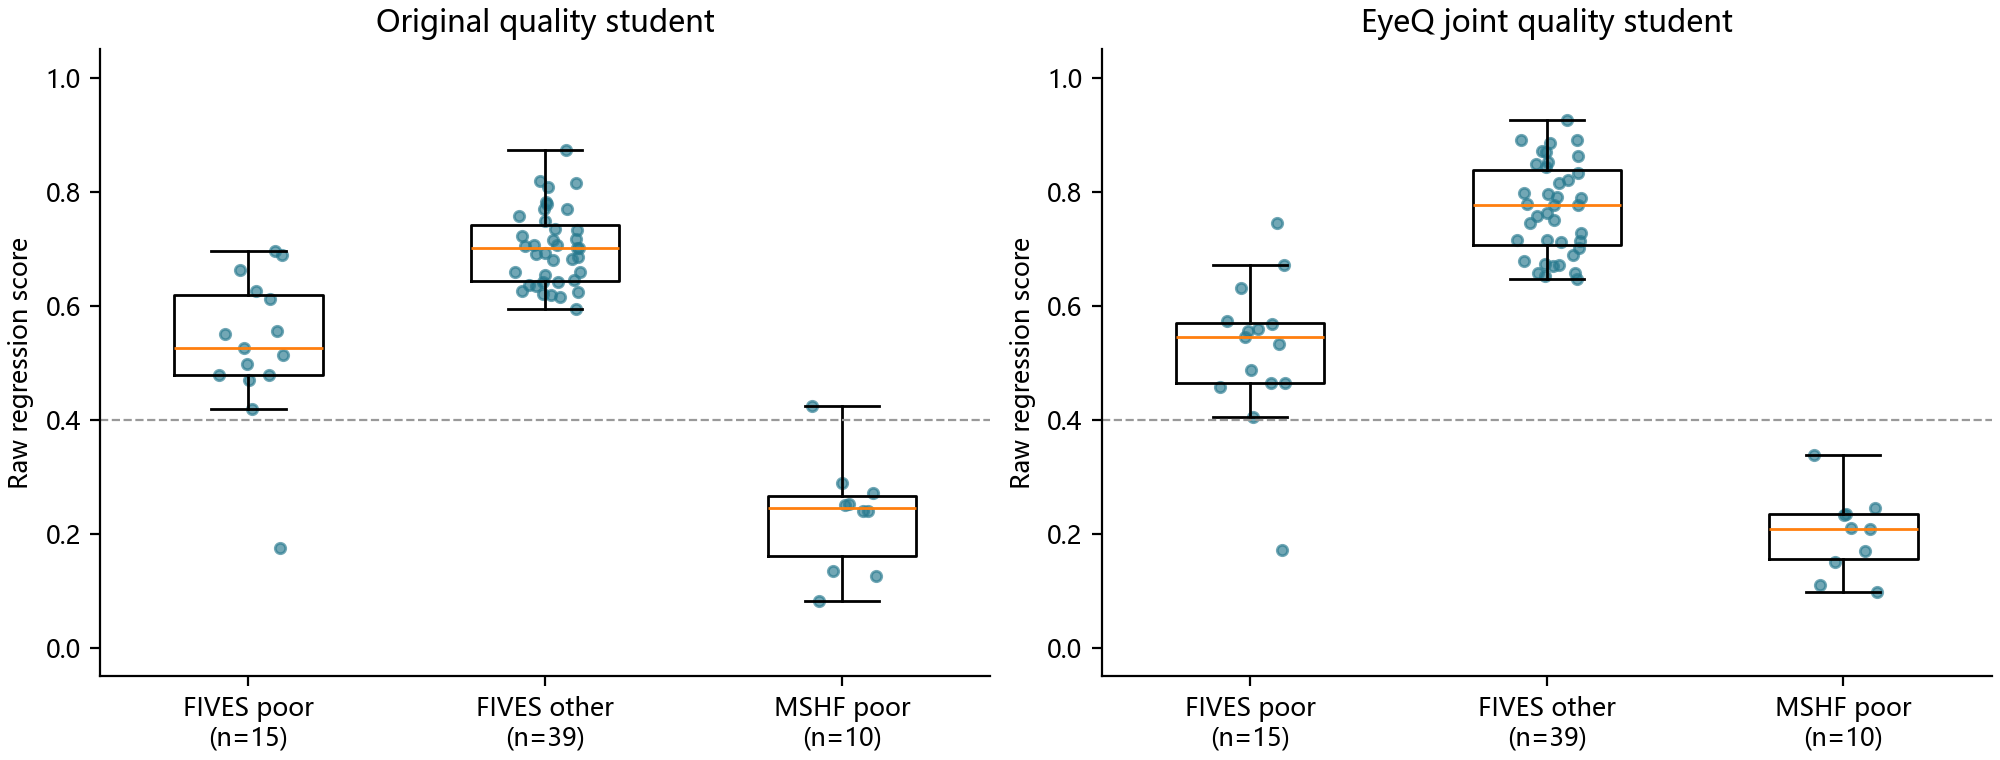
\includegraphics[keepaspectratio,alt={Raw scores from two quality models, grouped by source human grades}]{human-quality-scores.en.png}}
\caption{Raw scores from two quality models, grouped by source human
grades}
\end{figure}

Figure 2 uses 54 FIVES and ten MSHF photographs across model validation
and rule development. FIVES defines poor quality as at least one poor
dimension; MSHF uses official overall quality. Dots are photographs,
boxes span quartiles, and the central line is the median. The dashed 0.4
line aids numerical comparison and is not a human-grade threshold.

The original student's median q is 0.5261 for 15 poor-quality FIVES
images and 0.7008 for 39 other-quality images. Only 1/15 poor images
fall below 0.4. The ten poor-overall MSHF images have median 0.2453,
with 9/10 below 0.4. Within FIVES, low q distinguishes poor human
quality with AUROC 0.9026. These findings support differences in source
score scales and quality definitions rather than complete quality-model
failure. Whole-image quality also differs from visibility of the
optic-disc information needed for diagnosis.

An additional inference pass uses the EyeQ joint quality checkpoint
selected at epoch 17 on the same 4,099 development originals. Its FIVES
human-quality AUROC is 0.9641. Adding this score gives an error-model
AUROC of 0.8775, a difference of -0.0005 versus the p model, with a 95\%
interval {[}-0.0020, +0.0010{]}. Both quality models output raw
regression scores; the following comparison examines errors and misses
at matched review volume.

File hashes of both quality training cohorts were compared with these
disease development photographs: both exact-file intersections are zero.
This excludes byte-identical training photographs; other confirmed
relationships follow the frozen association audit.

\subsection{The shortage primarily concerns poor-quality
negatives}\label{the-shortage-primarily-concerns-poor-quality-negatives}

\begin{figure}[H]
\centering
\pandocbounded{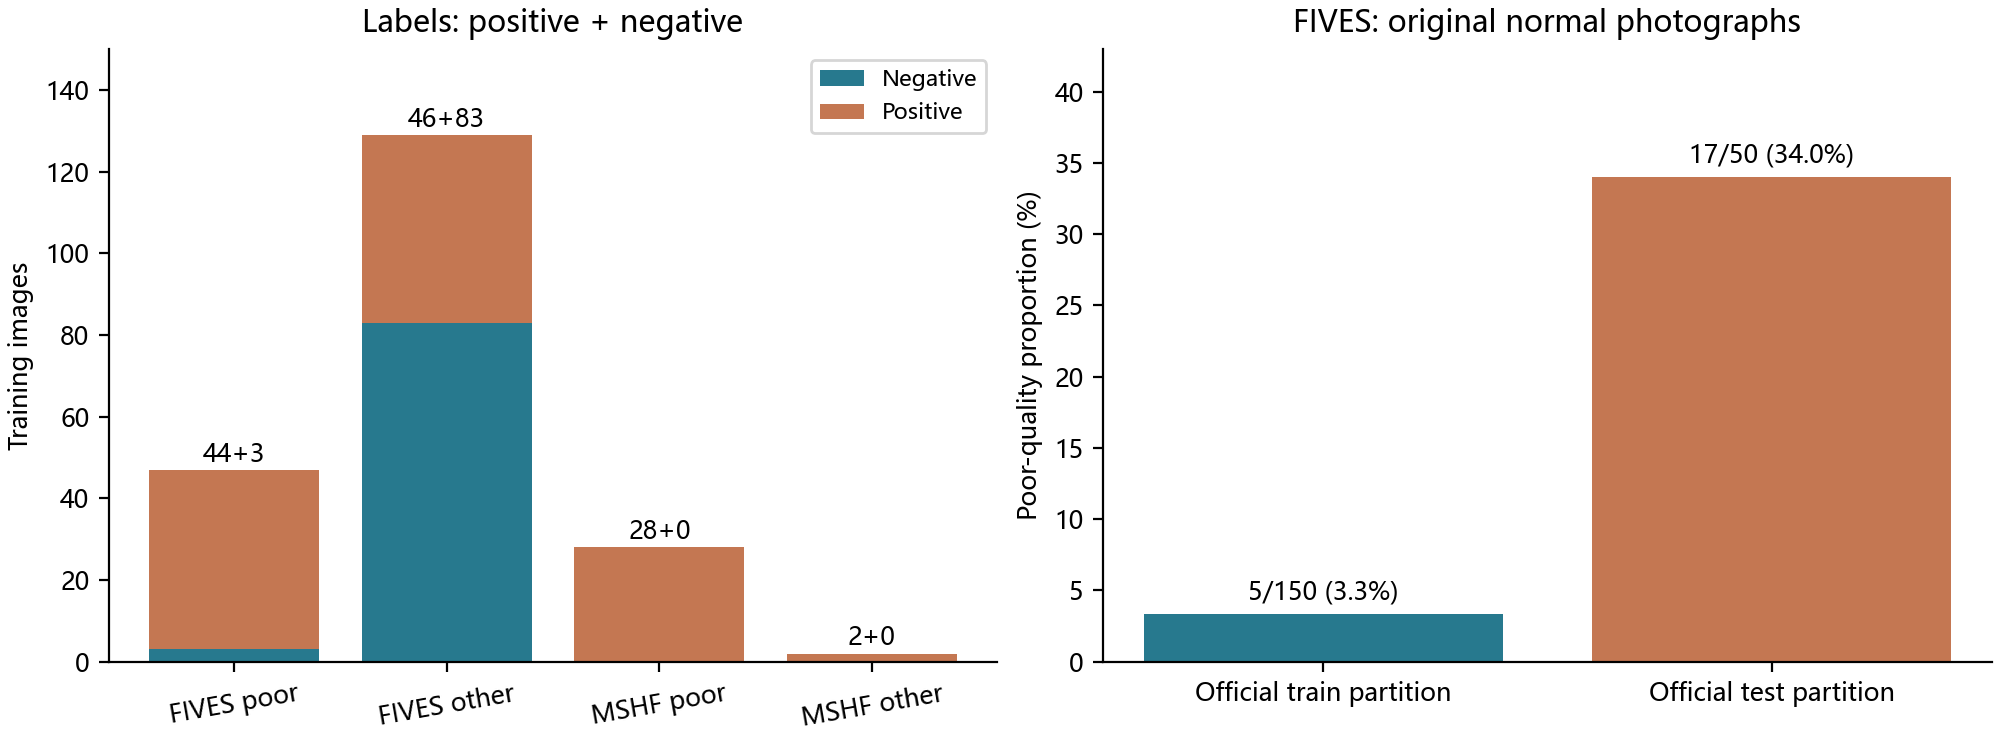
\includegraphics[keepaspectratio,alt={Disease-label composition by quality and the original FIVES partition difference}]{quality-label-composition.en.png}}
\caption{Disease-label composition by quality and the original FIVES
partition difference}
\end{figure}

Figure 3 uses the frozen training manifest on the left; labels above
bars are positive + negative counts. Poor-quality FIVES training
contains 44 positives and three negatives, while other quality contains
46 positives and 83 negatives. MSHF contributes 28 poor-quality
positives and no poor-quality negatives; its two other-quality images
are also positive. Of 75 poor-quality training photographs, 72 are
positive. The FIVES odds ratio associating poor quality with a positive
label is 26.46: positive-to-negative odds are about 26 times larger
among poor than other-quality training photographs. This composition may
let the model use source or quality cues; the current detections do not
establish recognition based solely on disease features. Repeated
sampling increases presentations of existing photographs: the previous
run presented real poor-quality positives 413 times and negatives only
ten times.

The right panel checks the original official FIVES quality workbook.
Among normal photographs, poor-quality prevalence is 5/150, or 3.3\%, in
its official training partition, versus 17/50, or 34.0\%, in its test
partition. This partly explains the shortage of poor-quality negatives
in development. The frozen rule-development set has seven poor FIVES
positives and five poor MSHF positives, with no poor negatives; model
validation contains only one poor FIVES negative. Detecting 12/12
positives therefore cannot estimate false alarms in this stratum or
establish stable quality robustness.

If 12 independent positive cases have zero misses, the exact one-sided
95\% upper bound on miss rate remains 22.1\%. Under the ideal zero-error
condition, at least 59 independent cases are needed to bring that bound
below 5\%; false-alarm precision requires a separate set of at least 59
independent negatives. At an error rate around 10\%, the usual
approximation requires about 139 cases for a 95\% interval half-width
near five percentage points. These are planning references for each
evaluated stratum, with positives and negatives counted separately;
linked photographs do not add independent cases.

All 26 photographs in the local MSHF Healthy worksheet have good overall
quality. The earlier audit excluded 20 as within-acquisition duplicates
and six as duplicates with conflicting identical-image labels. They
cannot directly provide new poor-quality negatives. Existing FIVES
test-role images remain reserved for final evaluation. Additional cases
should prioritize the same sources and acquisition conditions, reliable
negative disease labels, and real human quality annotations.
Other-disease folders do not establish glaucoma-negative status.

\subsection{Does q improve review
selection?}\label{does-q-improve-review-selection}

To reduce fitting and assessing a boundary on the same images, this
analysis uses five-fold linked-group cross-validation. All images from a
linked group stay in one fold. A low-complexity logistic error model is
trained on four folds and generates error-risk predictions for the
held-out fold. The p model uses log-odds of p, absolute log-odds, and a
squared term. The p,q model adds q and two interactions. Scaling is
fitted within each training fold. The disease model is already fixed;
this cross-validation evaluates the error-ranking model.

The following comparison selects the same 411/2,053 images, about 20\%,
for review. p uncertainty prioritizes scores nearest 0.5; low q
prioritizes the smallest q. The fitted models use out-of-fold
predictions. Image identifiers deterministically resolve tied scores.

\Needspace{9\baselineskip}
\begin{longtable}[]{@{}
  >{\raggedright\arraybackslash}p{(\linewidth - 8\tabcolsep) * \real{0.2000}}
  >{\raggedright\arraybackslash}p{(\linewidth - 8\tabcolsep) * \real{0.2000}}
  >{\raggedright\arraybackslash}p{(\linewidth - 8\tabcolsep) * \real{0.2000}}
  >{\raggedright\arraybackslash}p{(\linewidth - 8\tabcolsep) * \real{0.2000}}
  >{\raggedright\arraybackslash}p{(\linewidth - 8\tabcolsep) * \real{0.2000}}@{}}
\toprule\noalign{}
\begin{minipage}[b]{\linewidth}\raggedright
Ranking
\end{minipage} & \begin{minipage}[b]{\linewidth}\raggedright
Error AUROC
\end{minipage} & \begin{minipage}[b]{\linewidth}\raggedright
Errors selected / 208
\end{minipage} & \begin{minipage}[b]{\linewidth}\raggedright
Misses selected / 124
\end{minipage} & \begin{minipage}[b]{\linewidth}\raggedright
Unreviewed errors / images
\end{minipage} \\
\midrule\noalign{}
\endhead
\bottomrule\noalign{}
\endlastfoot
p uncertainty & 0.8772 & 145/208 & 86/124 & 63/1642 \\
Low q only & 0.5092 & 39/208 & 18/124 & 169/1642 \\
p error model & 0.8780 & 141/208 & 87/124 & 67/1642 \\
p,q error model & 0.8783 & 142/208 & 90/124 & 66/1642 \\
p, EyeQ q & 0.8775 & 145/208 & 90/124 & 63/1642 \\
\end{longtable}

\begin{figure}[H]
\centering
\pandocbounded{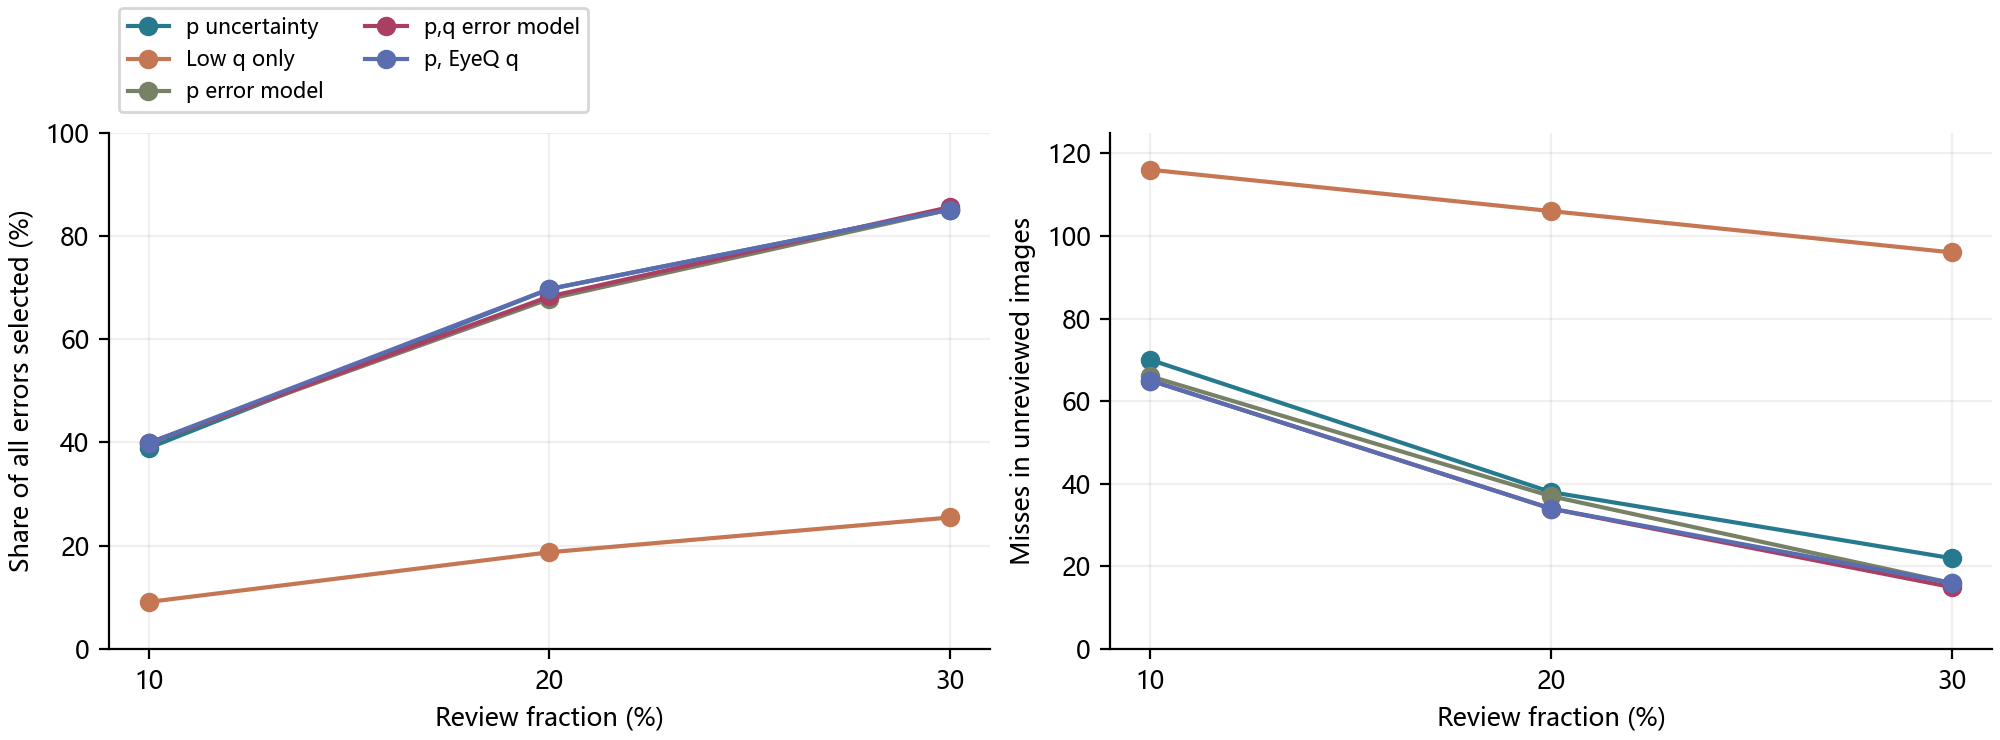
\includegraphics[keepaspectratio,alt={Errors selected and misses left unreviewed at different review volumes}]{review-comparison.en.png}}
\caption{Errors selected and misses left unreviewed at different review
volumes}
\end{figure}

Figure 4 shows the share of errors selected and misses remaining among
automatic outputs. Adding q changes error AUROC by only +0.00029 versus
the corresponding p model, with a paired linked-group 95\% interval
{[}−0.00158, +0.00225{]}. AUPRC summarizes error-selection precision and
recall: how many selected images are errors, and how many of all errors
are selected. It changes by +0.0067 {[}−0.0142, +0.0277{]}. At 20\%
review, q selects one additional error. Each case bootstrap reranks the
scores and selects the same number of images with both methods, giving a
95\% interval {[}-2, +7{]}. Adding source indicators also yields a small
change, and two other fold-assignment seeds show no material
improvement.

The error model using EyeQ scores selects 145 errors at about 20\%
review, including 90 misses. Compared with p uncertainty, it selects the
same number of total errors but four additional misses, reducing
unreviewed misses from 38 to 34. This tradeoff warrants further testing;
it is a development-data result and does not yet establish a stable
advantage.

These results establish p uncertainty as a necessary comparator while
testing q's additional information. Capacity matching is exploratory on
rule development and does not lock a deployment threshold. Bootstrap
intervals hold the generated out-of-fold predictions fixed, reflecting
case sampling rather than all uncertainty from refitting a boundary. The
table counts errors sent for review without assuming that real reviewers
always correct them.

\subsection{What the new training
tests}\label{what-the-new-training-tests}

The six conditions are original-data clean, expanded clean, 65\%
original-origin quota clean, current sampling with 50\% mixed
degradation, 65\% quota with 50\% mixed degradation, and 65\% quota with
50\% defocus-only degradation. Common seeds are 20261115, 20261116, and
20261117. Each EfficientNet-B0 starts from the same ImageNet weights and
uses 320-pixel input, batches up to 16, AdamW learning rate 0.0001, and
2,400 successful parameter updates. This budget does not mean 20
completed epochs. One successful update adjusts parameters using one
sampled batch. An epoch draws as many images as the training pool
contains, with repeats permitted by the sampler.

The original-data control uses 10,338 training photographs; the other
conditions use 15,480. Every 300 updates, the same 2,046
model-validation photographs are evaluated and full checkpoints plus
image predictions are saved. Selection uses the equal AUROC mean over
AIROGS, ODIR, Kaggle, LAG, and KEH, reducing the earlier influence of
four tiny sources carrying 36.4\% of the selection mean. Update-1,200
and update-2,400 weights remain available separately from the selected
checkpoint.

Within original and added origin pools, the 65\% quota retains
inverse-square-root source-class sampling. The quota is distributed
through consecutive draw positions, so truncated update budgets retain
approximately 65\% original-image presentations. The previous round
reduced original-source presentations from 19,186 to 9,484. This tests
whether restoring original-source presentations improves AIROGS and
ODIR; it adds no real poor-quality cases. Defocus-only and mixed
augmentation share application probability and image sampling sequence
to separate mechanisms.

The status snapshot was captured at 2026-11-15T06:28:42.791150+00:00.
Training budgets are complete for 2/18 runs and development evaluation
for 2/18. The current run is \texttt{seed20261115/quota65\_clean}, and
the driver state is \texttt{training}. A hidden background process
continues after this conversation; checkpoint recovery verifies input
fingerprints.

\Needspace{9\baselineskip}
\begin{longtable}[]{@{}lll@{}}
\toprule\noalign{}
Run & Latest evaluated update & Five-source validation AUROC mean \\
\midrule\noalign{}
\endhead
\bottomrule\noalign{}
\endlastfoot
seed20261115/expanded\_clean & 2400 & 0.9610 \\
seed20261115/original\_clean & 2400 & 0.8651 \\
seed20261115/quota65\_clean & 900 & 0.9462 \\
\end{longtable}

The following disease-classification AUROCs use the same
rule-development originals: AIROGS 773 (380 positives), ODIR 305 (28),
Kaggle 142 (95), LAG 481 (169), and KEH 153 (75). The checkpoint marked
selected was chosen on model validation.

\Needspace{9\baselineskip}
\begin{longtable}[]{@{}
  >{\raggedright\arraybackslash}p{(\linewidth - 12\tabcolsep) * \real{0.14285}}
  >{\raggedright\arraybackslash}p{(\linewidth - 12\tabcolsep) * \real{0.14285}}
  >{\raggedright\arraybackslash}p{(\linewidth - 12\tabcolsep) * \real{0.14285}}
  >{\raggedright\arraybackslash}p{(\linewidth - 12\tabcolsep) * \real{0.14285}}
  >{\raggedright\arraybackslash}p{(\linewidth - 12\tabcolsep) * \real{0.14285}}
  >{\raggedright\arraybackslash}p{(\linewidth - 12\tabcolsep) * \real{0.14285}}
  >{\raggedright\arraybackslash}p{(\linewidth - 12\tabcolsep) * \real{0.14285}}@{}}
\toprule\noalign{}
\begin{minipage}[b]{\linewidth}\raggedright
Run
\end{minipage} & \begin{minipage}[b]{\linewidth}\raggedright
Updates
\end{minipage} & \begin{minipage}[b]{\linewidth}\raggedright
AIROGS
\end{minipage} & \begin{minipage}[b]{\linewidth}\raggedright
ODIR
\end{minipage} & \begin{minipage}[b]{\linewidth}\raggedright
Kaggle
\end{minipage} & \begin{minipage}[b]{\linewidth}\raggedright
LAG
\end{minipage} & \begin{minipage}[b]{\linewidth}\raggedright
KEH
\end{minipage} \\
\midrule\noalign{}
\endhead
\bottomrule\noalign{}
\endlastfoot
20261115 / original clean & 1200 & 0.9743 & 0.9375 & 0.9888 & 0.9426 &
0.5889 \\
20261115 / original clean & 1800 (selected) & 0.9793 & 0.9531 & 0.9892 &
0.9434 & 0.6431 \\
20261115 / original clean & 2400 & 0.9796 & 0.9381 & 0.9937 & 0.9450 &
0.5593 \\
20261115 / expanded clean & 1200 & 0.9644 & 0.9569 & 0.9747 & 0.9893 &
0.9443 \\
20261115 / expanded clean & 2400 (selected) & 0.9670 & 0.9474 & 0.9789 &
0.9907 & 0.9410 \\
\end{longtable}

For the first seed, 20261115, at the same 2,400-update budget, expansion
changes disease AUROC by -0.0125 on AIROGS, +0.0457 on LAG, +0.3817 on
KEH, and +0.0093 on ODIR. ODIR differs in direction from the previous
update-1,200 comparison; seeds and budgets also differ between rounds,
so its effect should be assessed after all three common seeds complete.
The original-data control still misses five of the 12 poor-quality
development positives, while expanded clean misses none; this stratum
still has no negatives.

A further check uses the update-2,400 disease weights, the same
rule-development photographs, and the original quality student scores to
rank errors. The following compares low q and p uncertainty separately
without refitting a p,q boundary.

\Needspace{9\baselineskip}
\begin{longtable}[]{@{}
  >{\raggedright\arraybackslash}p{(\linewidth - 6\tabcolsep) * \real{0.2500}}
  >{\raggedright\arraybackslash}p{(\linewidth - 6\tabcolsep) * \real{0.2500}}
  >{\raggedright\arraybackslash}p{(\linewidth - 6\tabcolsep) * \real{0.2500}}
  >{\raggedright\arraybackslash}p{(\linewidth - 6\tabcolsep) * \real{0.2500}}@{}}
\toprule\noalign{}
\begin{minipage}[b]{\linewidth}\raggedright
Run
\end{minipage} & \begin{minipage}[b]{\linewidth}\raggedright
Errors / images
\end{minipage} & \begin{minipage}[b]{\linewidth}\raggedright
Low-q error AUROC
\end{minipage} & \begin{minipage}[b]{\linewidth}\raggedright
p uncertainty error AUROC
\end{minipage} \\
\midrule\noalign{}
\endhead
\bottomrule\noalign{}
\endlastfoot
20261115 / original clean & 264/2053 & 0.5412 & 0.8301 \\
20261115 / expanded clean & 154/2053 & 0.5375 & 0.8717 \\
\end{longtable}

Latest validation rows report their corresponding saved update.
Available development AUROCs are shown by source and update checkpoint.
Variation across training seeds and sampling or degradation conclusions
will be summarized after all three seeds finish. Final held-out testing
waits until models, classification thresholds, and review rules are
fixed.

\subsection{Reproduction and evidence}\label{reproduction-and-evidence}

\href{quality-error-analysis.json}{Analysis data} ·
\href{training-snapshot.json}{Training snapshot} ·
\href{../../../tools/analyze_quality_errors_20261115.py}{Analysis
program} ·
\href{../../../tools/report_quality_training_20261115.py}{Report
generator} ·
\href{../../../tools/start_followup_experiments_20261115.ps1}{Training
launcher} ·
\href{../../../runs/followup_20261115/pipeline/status.json}{Live
execution status}

Image-level joins and out-of-fold risks are stored locally under
\texttt{runs/followup\_20261115/error\_ranking/}. The new run directory
holds quality inference evidence, the plan, every validation checkpoint,
and training logs. Report data retain input SHA256 hashes. Chinese and
English Markdown, PDF, LaTeX, and figures share this dated directory;
historical experiments remain intact.

\end{document}
